\begin{figure}[H]
  \centering
  \textbf{Varying  }
  \newline
  \newline
  \pgfplotsset{
    scale only axis,
    legend style={at={(0,0.8)}, anchor=west, font=\tiny},
    xmin=7,
  }
  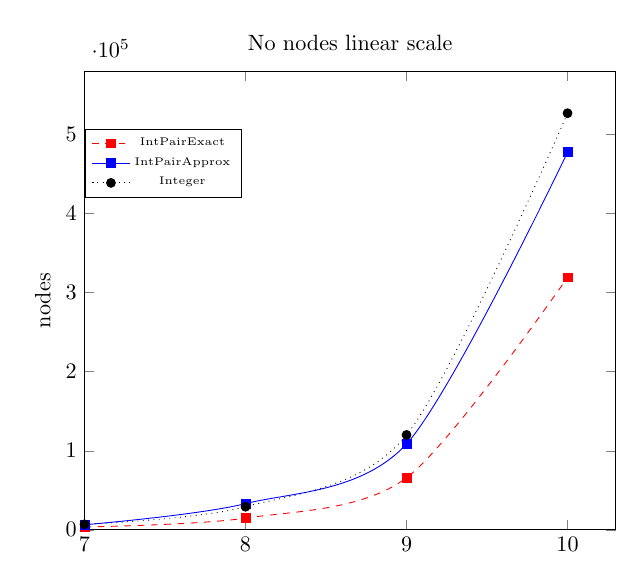
\begin{tikzpicture} [scale=0.8]
    \begin{axis}[
        title=No nodes linear scale,
        ylabel=nodes,
        xtick=data,
        ymin=0, 
        xlabel= ]
      \addplot[smooth,mark=square*, mark options={solid},red, dashed]
      coordinates{ (7, 3612) (8, 14817) (9, 65810) (10, 319263)
      }; \label{ie_plot} \addlegendentry{IntPairExact}
      \addplot[smooth,mark=square*, mark options={solid},blue]
      coordinates{ (7, 6374) (8, 33149) (9, 108671) (10, 477582)
      }; \label{ia_plot} \addlegendentry{IntPairApprox}
      \addplot[smooth,mark=*,mark options={solid},black, dotted]
      coordinates{ (7, 6999) (8, 29162) (9, 119996) (10, 526972)
      }; \label{int_plot} \addlegendentry{Integer}
    \end{axis}
  \end{tikzpicture}
  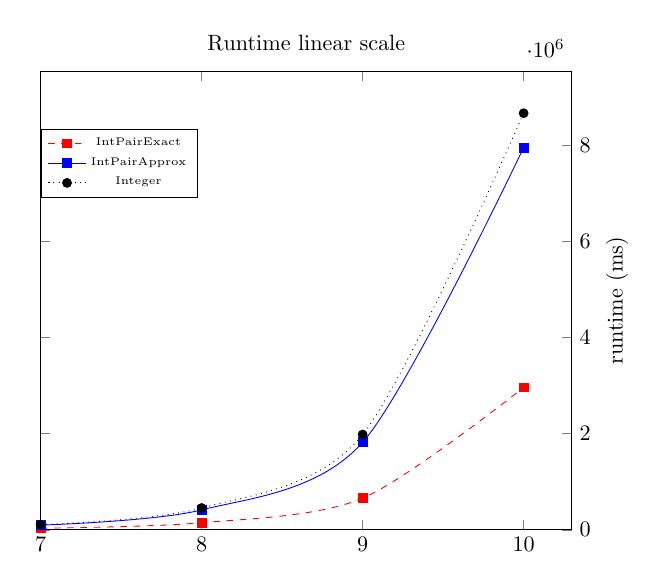
\begin{tikzpicture} [scale=0.8]
    \begin{axis}[
        yticklabel pos=right,
        xtick=data,
        title=Runtime linear scale,
        ylabel=runtime (ms),
        xlabel=,
        ymin=0, ]
      \addplot[smooth,mark=square*,mark options={solid},red, dashed]
      coordinates{ (7,33465) (8,146201) (9,658312) (10,2959824)
      }; \label{IntPairExact Run}
      \addplot[smooth,mark=square*,mark options={solid},blue]
      coordinates{ (7,97813) (8,414505) (9,1819264) (10,7950138)
      }; \label{IntPairApprox Run}
      \addplot[smooth,mark=*,mark options={solid},black, dotted]
      coordinates{ (7,107122) (8,453696) (9,1981650) (10,8664862)
      }; \label{IntegerRun}
      \addlegendentry{IntPairExact}
      \addlegendentry{IntPairApprox}
      \addlegendentry{Integer}
    \end{axis}
  \end{tikzpicture}

  
\begin{tikzpicture}[scale=1.4]
    \draw[very thick] (-4,0) -- (4,0);
    \draw[draw=white] (-5,-0.2) -- (5,-0.2);
  \end{tikzpicture}


  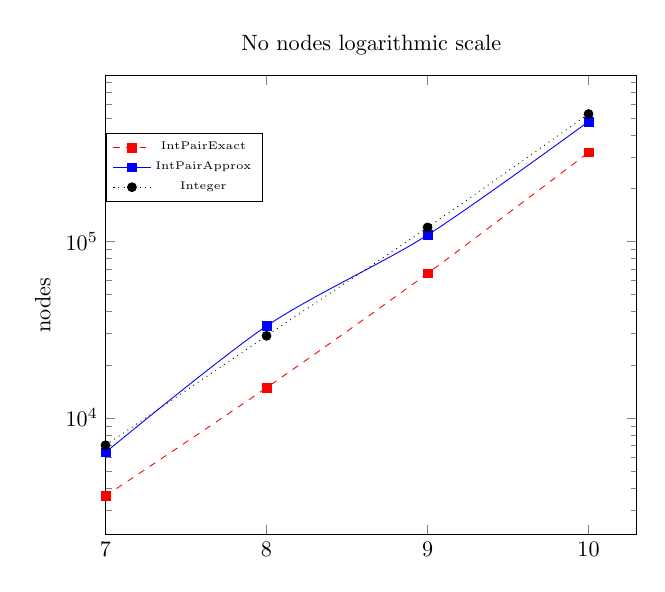
\begin{tikzpicture} [scale=0.8]
    \begin{semilogyaxis}[
        title=No nodes logarithmic scale,
        ylabel=nodes,
        xtick=data,
        ymin=0, 
        xlabel= ]
     \addplot[smooth,mark=square*, mark options={solid},red, dashed]
      coordinates{ (7, 3612) (8, 14817) (9, 65810) (10, 319263)
      }; \label{ie_plot} \addlegendentry{IntPairExact}
      \addplot[smooth,mark=square*, mark options={solid},blue]
      coordinates{ (7, 6374) (8, 33149) (9, 108671) (10, 477582)
      }; \label{ia_plot} \addlegendentry{IntPairApprox}
      \addplot[smooth,mark=*,mark options={solid},black, dotted]
      coordinates{ (7, 6999) (8, 29162) (9, 119996) (10, 526972)
      }; \label{int_plot} \addlegendentry{Integer}

    \end{semilogyaxis}
  \end{tikzpicture}
  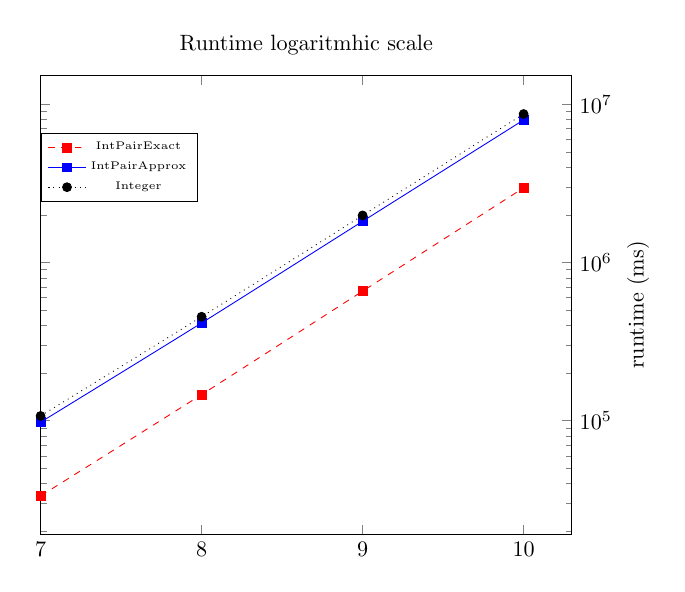
\begin{tikzpicture} [scale=0.8]
    \begin{semilogyaxis}[
        title=Runtime logaritmhic scale,
        yticklabel pos=right,
        xtick=data,
        ylabel=runtime (ms),
        xlabel=,
        ymin=0,  ]
      \addplot[smooth,mark=square*,mark options={solid},red, dashed]
      coordinates{ (7,33465) (8,146201) (9,658312) (10,2959824)
      }; \label{IntPairExact Run}
      \addplot[smooth,mark=square*,mark options={solid},blue]
      coordinates{ (7,97813) (8,414505) (9,1819264) (10,7950138)
      }; \label{IntPairApprox Run}
      \addplot[smooth,mark=*,mark options={solid},black, dotted]
      coordinates{ (7,107122) (8,453696) (9,1981650) (10,8664862)
      }; \label{IntegerRun}
      \addlegendentry{IntPairExact}
      \addlegendentry{IntPairApprox}
      \addlegendentry{Integer}
    \end{semilogyaxis}
  \end{tikzpicture}
  \caption{{Caption}}\label{fig:}
\end{figure}
